%!TEX root = ../main.tex
\chapter{Krav}

I dette afsnit beskrives de opstillede krav for AVS. På \ref{photo:UseCD} ses det færdige Use case diagram over systemet, der ligger til grund for de funktionelle krav.

\begin{figure}[H]
	\centering
	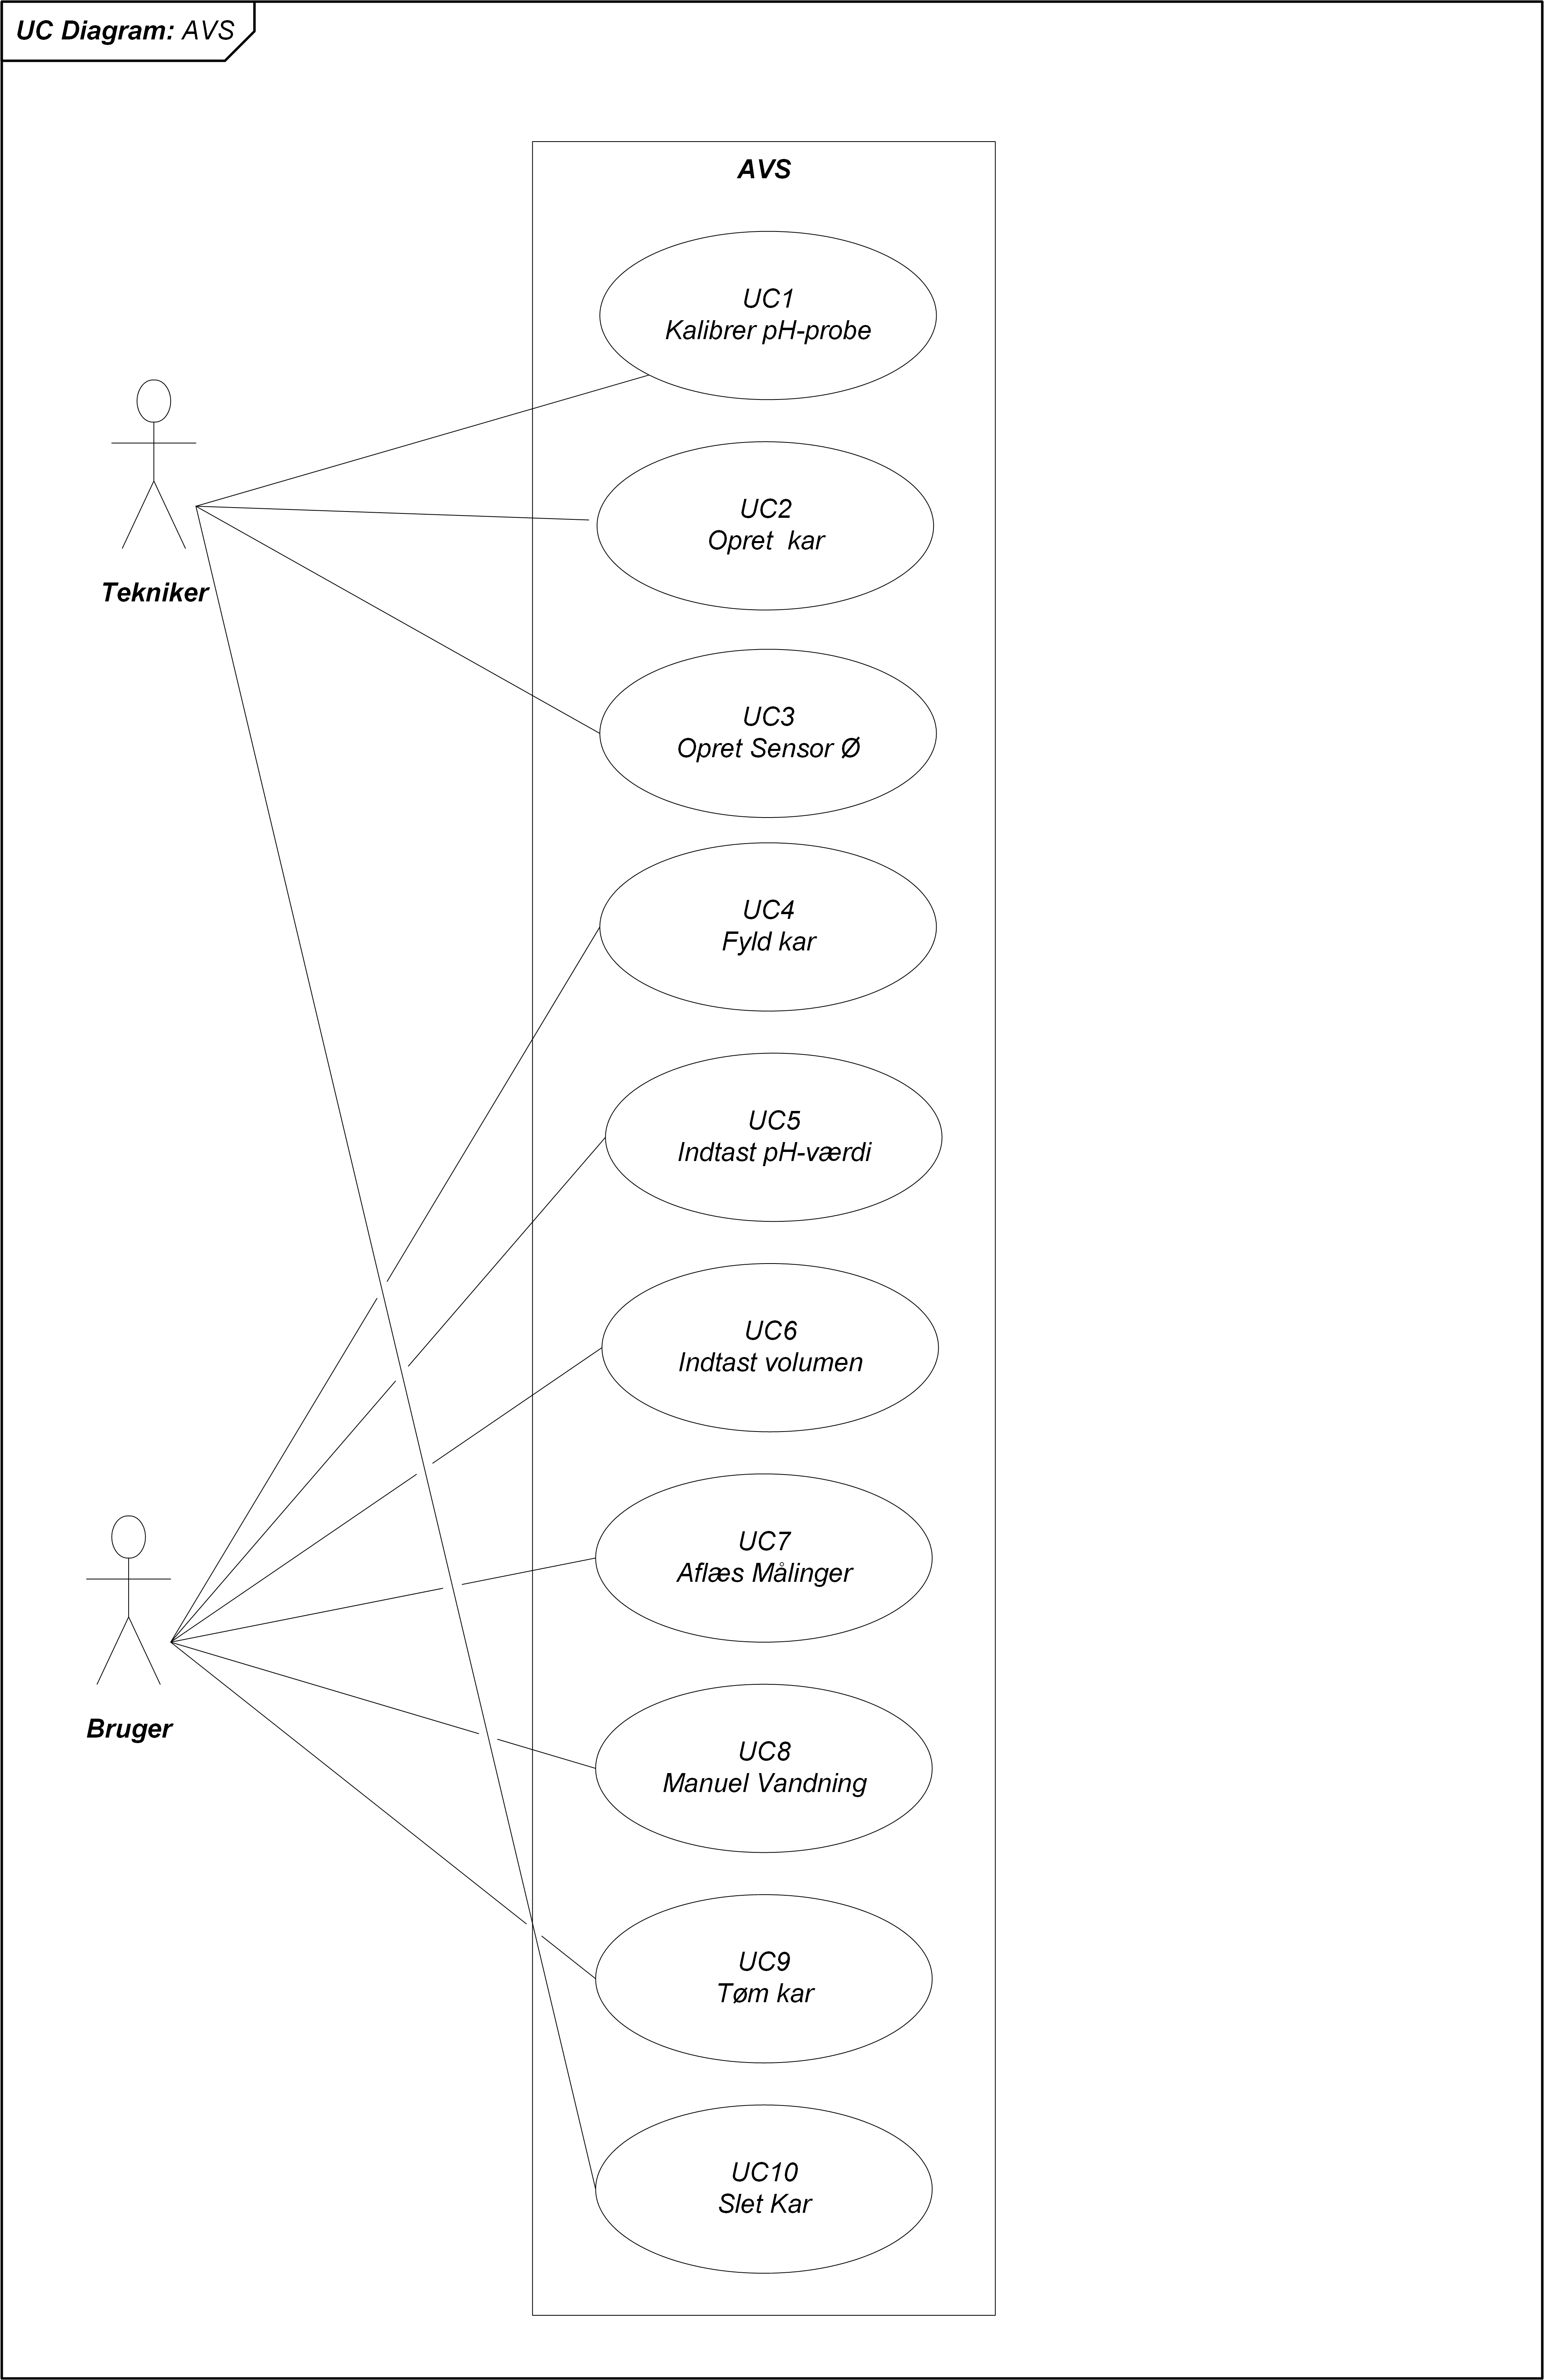
\includegraphics[scale=0.6]{Krav/Billeder/AVS_UseCases}
	\caption{AVS Use case diagram}
	\label{photo:UseCD}
\end{figure}

Herunder findes en kort beskrivelse af de enkelte use cases.\newline 
For yderlige detaljer henvises til Projektdokumentationens afsnit 1.2 "Use Cases".

\newpage
\textbf{Use Case 1 - Kalibrer pH-Probe}\newline
Denne use case har til formål at lade Tekniker kalibrere den pH-probe der er tilsluttet et givent kar. Denne use case skal køres hver gang systemet startes op.\newline

\textbf{Use Case 2 - Opret kar}\newline
Denne use case har til formål at lade Tekniker oprette et nyt Kar til systemet, dette udføres fra Gui'en i brugerens webbrowser. \newline

\textbf{Use Case 3 - Opret Sensor Ø}\newline
Denne use case har til formål at lade Tekniker oprette en ny SensorØ til systemet, dette udføres fra Gui'en i brugerens web-browser.\newline

\textbf{Use Case 4 - Fyld kar}\newline
Denne use case har til formål at lade Bruger åbne for indløbsventilen og fylde karet med vand.\newline

\textbf{Use Case 5 - Indtast pH-værdi}\newline
Denne use case har til formål at lade Bruger indtaste en ønsket pH-værdi via Gui'en. Herefter justerer systemet Gødning/vand indtil den indtastede pH-værdi er opnået. \newline

\textbf{Use Case 6 - Indtast volumen}\newline
Denne use case har til formål at lade Bruger indtaste en ønsket volumen via Gui'en. Herefter justerer systemet ind- og afløbsventiler indtil den indtastede volumen er opnået.\newline

\textbf{Use Case 7 - Aflæs målinger}\newline
Denne use case har til formål at lade Bruger tilgå de tilkoblede kar via Gui'en og aflæse ønskede data.\newline

\textbf{Use Case 8 - Manuel vanding}\newline
Denne use case har til formål at lade Bruger, manuelt tilføre vand til gromediet.\newline

\textbf{Use Case 9 - Tøm kar}\newline
Denne use case har til formål at lade Bruger åbne for afløbsventilen, tænde pumpen og tømme karet for vand.\newline

\textbf{Use Case 10 - Slet kar}\newline
Denne use case har til formål at lade Tekniker, via Gui'en slette et givent kar fra systemet.\newline


Derudover er følgende use cases tilføjet systemet, dog på ikke-fullydressed basis. For yderlige detaljer om de enkelte use cases refereres til Projektdokumentationens afsnit 1.3 "Ikke fully dressed Use Cases"\\\

\textbf{Use Case 11 - Doser pH-væske}\newline
Denne use case har til formål at Bruger får mulighed for, manuelt at dosere pH-væske via en doseringspumpe indtil den
ønskede pH-værdi er opnået.\newline

\textbf{Use Case 12 - Automatisk vanding}\newline 
Denne use case har til formål at lade vandingen ske automatisk, baseret på den målte jordfugtighed.\newline

\textbf{Use Case 13 - Alarm}\newline 
Denne use case har til formål at lade Systemet afgive en alarm hvis de brugerdefinerede grænseværdier (jordfugtighed, pH-værdi og volumen) overskrides.\newline

\textbf{Use Case 14 - Ugeplan}\newline
Denne use case giver Bruger mulighed for at indtaste en ugeplan for styring af dosering af pH-væske
og vand til gromediet.\newline

\textbf{Use Case 15 - Udprint log}\newline 
Denne use case giver Bruger mulighed for at få udprintet en log over de hændelser der er forekommet i systemet, herunder optaget sensordata samt dosering af vand.\newline


For at sikre kvaliteten af det færdige produkt, er der opstillet en række ikke funktionelle krav. Disse beskrives kort herunder, for yderligere detaljer henvises til Projektdokumentationens afsnit 1.4 "Ikke funktionelle krav"

De ikke-funktionelle krav er inddelt i 3 undergrupper: 

\begin{itemize}
	\item	Brugervenlighed
	\item	Systembetingelser
	\item	Ydelse
\end{itemize}

Kravene under brugervenlighed baserer sig på at systemet skal kunne kører på en "standard" PC og kunne tilgås igennem normal webbrowser. Derudover skal systemet både kunne tilgås over lokalt netværk samt over www.\newline
Under Systembetingelser opsættes de miljømæssige omstændigheder under hvilke hvor systemet skal kunne opererer.\newline 
Ydelse opsætter de tider og grænseværdier for fyldning og tømning af systemet, samt for dosering af gødning og vand til gromediet.